% ============================================================
%  Sleep Monitor — Beamer Presentation
%  Compile: latexmk -pdf main.tex   (or pdflatex twice)
% ============================================================
\documentclass[aspectratio=169,10pt]{beamer}
\usetheme{metropolis}

\usepackage[T1]{fontenc}
\usepackage{tikz}
\usepackage{fontawesome5}
\usepackage{xcolor}
\usetikzlibrary{calc, arrows.meta, positioning}

% ── COLORS ────────────────────────────────────────────────────
\definecolor{sleepnavy}{HTML}{0B2545}
\definecolor{sleepteal}{HTML}{0D9488}
\definecolor{sleepmid}{HTML}{1565C0}
\definecolor{sleepbg}{HTML}{F8FAFC}
\definecolor{hwblue}{HTML}{1E88E5}
\definecolor{cloudteal}{HTML}{0D9488}
\definecolor{purplephone}{HTML}{7C3AED}
\definecolor{warnambr}{HTML}{D97706}
\definecolor{sleepgray}{HTML}{64748B}

% ── THEME ─────────────────────────────────────────────────────
\setbeamercolor{palette primary}{bg=sleepnavy}
\setbeamercolor{alerted text}{fg=white}
\setbeamercolor{progress bar}{fg=sleepteal, bg=sleepnavy!40}
\setbeamercolor{title separator}{fg=sleepteal}
\setbeamercolor{frametitle}{bg=sleepnavy, fg=white}
\setbeamercolor{background canvas}{bg=sleepbg}
\setbeamercolor{normal text}{fg=sleepnavy}
\setbeamercolor{block title alerted}{fg=white, bg=sleepteal}
\setbeamercolor{block body alerted}{fg=sleepnavy, bg=sleepteal!12}

\metroset{block=fill, progressbar=foot, titleformat=regular}

\setbeamerfont{title}{size=\Huge, series=\bfseries}
\setbeamerfont{subtitle}{size=\large}
\setbeamerfont{frametitle}{size=\large, series=\bfseries}

% ── IMAGE PLACEHOLDER ─────────────────────────────────────────
%  \imgbox{width_cm}{height_cm}{color}{label}
\newcommand{\imgbox}[4]{%
  \begin{tikzpicture}
    \fill[#3!10, rounded corners=7pt] (0,0) rectangle (#1,-#2);
    \draw[#3, line width=1.2pt, dashed, rounded corners=7pt]
      (0,0) rectangle (#1,-#2);
    \node[#3!70!black, font=\small\itshape, align=center,
          text width={#1 cm}]
      at ($(0,0)!0.5!(#1,-#2)$) {#4};
  \end{tikzpicture}%
}

% ── META ──────────────────────────────────────────────────────
\title{Sleep Monitor}
\subtitle{IoT-Based Sleep Monitoring \& Therapy System}
\author{Miguel Flor $\cdot$ Bernardo Prioste}
\institute{IoT \& Mobile Systems --- 2025/26}
\date{}

% ══════════════════════════════════════════════════════════════
\begin{document}

% ── 1. TITLE ──────────────────────────────────────────────────
\begin{frame}
  \maketitle
\end{frame}

% ── 2. THE PROBLEM ────────────────────────────────────────────
\begin{frame}{The Problem}
  \vspace{0.3em}
  \begin{columns}[c]
    \begin{column}{0.54\textwidth}
      \begin{itemize}
        \setlength\itemsep{1.2em}
        \item[\textcolor{sleepteal}{\large\faHospital}]
          \textbf{Sleep disorders} are prevalent in long-term clinical care,
          impacting patient recovery and wellbeing
        \item[\textcolor{sleepteal}{\large\faExclamationTriangle}]
          \textbf{Intrusive monitoring} disrupts sleep and provides limited
          real-time therapeutic insight
        \item[\textcolor{sleepteal}{\large\faTimes}]
          \textbf{No remote therapy control} — medical staff must physically
          intervene at night to adjust treatment
      \end{itemize}
    \end{column}
    \begin{column}{0.42\textwidth}
      \centering
      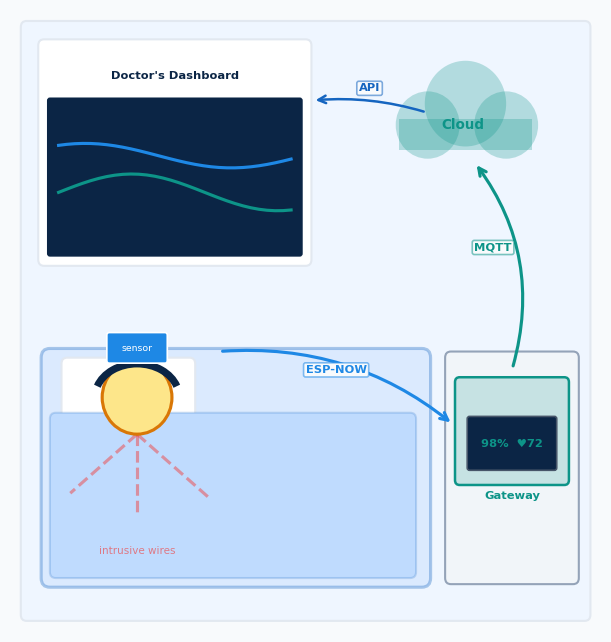
\includegraphics[width=\linewidth]{images/clinical_ward.png}
    \end{column}
  \end{columns}
\end{frame}

% ── 3. OUR SOLUTION ───────────────────────────────────────────
\begin{frame}{Our Solution}
  \vspace{0.3em}
  \begin{columns}[c]
    \begin{column}{0.54\textwidth}
      {\large A connected IoT ecosystem that:}\\[0.8em]
      \begin{itemize}
        \setlength\itemsep{0.9em}
        \item[\textcolor{sleepteal}{\large\faHeartbeat}]
          \textbf{Monitors} SpO\textsubscript{2}, heart rate \& movement
          in real time
        \item[\textcolor{sleepteal}{\large\faVolumeUp}]
          \textbf{Delivers} non-invasive sleep therapy via
          \emph{bone conduction} sound waves
        \item[\textcolor{sleepteal}{\large\faRss}]
          \textbf{Transmits} data reliably to the cloud via ESP-NOW + MQTT
        \item[\textcolor{sleepteal}{\large\faDesktop}]
          \textbf{Empowers} clinicians with a live dashboard
          \& remote therapy control
      \end{itemize}
    \end{column}
    \begin{column}{0.42\textwidth}
      \centering
      % ── System overview: 4-card hero ───────────────────────
      \begin{tikzpicture}
        % Background
        \fill[sleepnavy!5, rounded corners=7pt] (0,0) rectangle (5.4,-5.6);

        % ── Q1: Headband (top-left) ─────────────────────────
        \begin{scope}
          \clip[rounded corners=5pt] (0.1,-0.1) rectangle (2.3,-2.3);
          \fill[hwblue!7]  (0.1,-0.1) rectangle (2.3,-2.3);
          \fill[hwblue]    (0.1,-0.1) rectangle (2.3,-0.65);
        \end{scope}
        \draw[hwblue!25, line width=0.6pt, rounded corners=5pt]
          (0.1,-0.1) rectangle (2.3,-2.3);
        \node[white,          font=\tiny\bfseries] at (1.2,-0.375)
          {\faHeadphones\enspace Headband};
        \node[hwblue!80,      font=\large]         at (1.2,-1.12)
          {\faHeadphones};
        \node[hwblue!80!black,font=\tiny,align=center] at (1.2,-1.85)
          {MPU-6050 · MAX30102\\Bone Conduction};

        % ── Q2: Gateway (top-right) ─────────────────────────
        \begin{scope}
          \clip[rounded corners=5pt] (3.1,-0.1) rectangle (5.3,-2.3);
          \fill[cloudteal!7] (3.1,-0.1) rectangle (5.3,-2.3);
          \fill[cloudteal]   (3.1,-0.1) rectangle (5.3,-0.65);
        \end{scope}
        \draw[cloudteal!25, line width=0.6pt, rounded corners=5pt]
          (3.1,-0.1) rectangle (5.3,-2.3);
        \node[white,             font=\tiny\bfseries] at (4.2,-0.375)
          {\faServer\enspace Gateway};
        \node[cloudteal!80,      font=\large]         at (4.2,-1.12)
          {\faServer};
        \node[cloudteal!80!black,font=\tiny,align=center] at (4.2,-1.85)
          {ESP32 · OLED Display\\Wi-Fi · Bluetooth};

        % ── Q3: Cloud (bottom-left) ─────────────────────────
        \begin{scope}
          \clip[rounded corners=5pt] (0.1,-3.3) rectangle (2.3,-5.5);
          \fill[sleepmid!7] (0.1,-3.3) rectangle (2.3,-5.5);
          \fill[sleepmid]   (0.1,-3.3) rectangle (2.3,-3.85);
        \end{scope}
        \draw[sleepmid!25, line width=0.6pt, rounded corners=5pt]
          (0.1,-3.3) rectangle (2.3,-5.5);
        \node[white,            font=\tiny\bfseries] at (1.2,-3.575)
          {\faCloud\enspace Cloud Backend};
        \node[sleepmid!80,      font=\large]         at (1.2,-4.3)
          {\faCloud};
        \node[sleepmid!80!black,font=\tiny,align=center] at (1.2,-5.05)
          {MQTT · Database\\Backend API};

        % ── Q4: Dashboard (bottom-right) ─────────────────────
        \begin{scope}
          \clip[rounded corners=5pt] (3.1,-3.3) rectangle (5.3,-5.5);
          \fill[sleepnavy!7] (3.1,-3.3) rectangle (5.3,-5.5);
          \fill[sleepnavy]   (3.1,-3.3) rectangle (5.3,-3.85);
        \end{scope}
        \draw[sleepnavy!30, line width=0.6pt, rounded corners=5pt]
          (3.1,-3.3) rectangle (5.3,-5.5);
        \node[white,              font=\tiny\bfseries] at (4.2,-3.575)
          {\faDesktop\enspace Dashboard};
        \node[sleepnavy!75,       font=\large]         at (4.2,-4.3)
          {\faDesktop};
        \node[sleepnavy!80!black, font=\tiny,align=center] at (4.2,-5.05)
          {Real-time Vitals\\Remote Therapy};

        % ── Center label ─────────────────────────────────────
        \node[sleepnavy!35, font=\tiny\itshape, align=center] at (2.7,-2.8)
          {Sleep\\Monitor};

        % ── Arrows ───────────────────────────────────────────
        % Q1 → Q2: ESP-NOW
        \draw[->, >=Stealth, hwblue!70, line width=0.9pt]
          (2.3,-1.15) -- (3.1,-1.15)
          node[midway, above, font=\tiny\bfseries, hwblue!70] {ESP-NOW};
        % Q2 → Q4: MQTT
        \draw[->, >=Stealth, cloudteal!70, line width=0.9pt]
          (4.2,-2.3) -- (4.2,-3.3)
          node[midway, right, font=\tiny\bfseries, cloudteal!70] {MQTT};
        % Q4 → Q3: Web API
        \draw[->, >=Stealth, sleepnavy!50, line width=0.9pt]
          (3.1,-4.4) -- (2.3,-4.4)
          node[midway, above, font=\tiny\bfseries, sleepnavy!50] {API};
        % Q3 → Q1: Therapy (feedback loop, dashed)
        \draw[->, >=Stealth, sleepmid!60, line width=0.8pt, dashed]
          (1.2,-3.3) -- (1.2,-2.3)
          node[midway, left, font=\tiny\bfseries, sleepmid!55] {Therapy};
      \end{tikzpicture}
    \end{column}
  \end{columns}
\end{frame}

% ── 4. SYSTEM ARCHITECTURE ────────────────────────────────────
\begin{frame}{System Architecture}
  \centering
  \vspace{0.5em}
  \begin{tikzpicture}[
    hw/.style    = {rectangle, rounded corners=5pt,
                    draw=hwblue, fill=hwblue!12,
                    text width=2.0cm, align=center, minimum height=1.15cm,
                    font=\footnotesize\bfseries, text=sleepnavy},
    cloud/.style = {rectangle, rounded corners=5pt,
                    draw=cloudteal, fill=cloudteal!12,
                    text width=2.0cm, align=center, minimum height=1.15cm,
                    font=\footnotesize\bfseries, text=sleepnavy},
    phone/.style = {rectangle, rounded corners=5pt,
                    draw=purplephone, fill=purplephone!12,
                    text width=2.0cm, align=center, minimum height=1.15cm,
                    font=\footnotesize\bfseries, text=sleepnavy},
    arr/.style   = {->, >=Stealth, line width=1.3pt},
    lbl/.style   = {font=\tiny\bfseries, fill=sleepbg,
                    inner sep=2pt, rounded corners=2pt}
  ]
    \node[hw]    (hb)  at (0,   0)   {\large\faHeadphones\\[3pt]Wearable\\Headband};
    \node[hw]    (gw)  at (3.0, 0)   {\large\faServer\\[3pt]Gateway\\Device};
    \node[cloud] (cl)  at (6.0, 0)   {\large\faCloud\\[3pt]Cloud\\Backend};
    \node[cloud] (doc) at (9.0, 0)   {\large\faDesktop\\[3pt]Doctor\\Dashboard};
    \node[phone] (ph)  at (3.0,-2.3) {\large\faMobile\\[3pt]Smartphone};

    \draw[arr, hwblue]           (hb) -- node[lbl, above]{ESP-NOW}   (gw);
    \draw[arr, cloudteal]        (gw) -- node[lbl, above]{MQTT}      (cl);
    \draw[arr, cloudteal]        (cl) -- node[lbl, above]{Web API}   (doc);
    \draw[arr, purplephone, <->] (ph) -- node[lbl, right]{Bluetooth} (gw);
  \end{tikzpicture}
\end{frame}

% ── 5. WEARABLE HEADBAND ──────────────────────────────────────
\begin{frame}{Hardware — Wearable Headband}
  \begin{columns}[c]
    \begin{column}{0.42\textwidth}
      \centering
      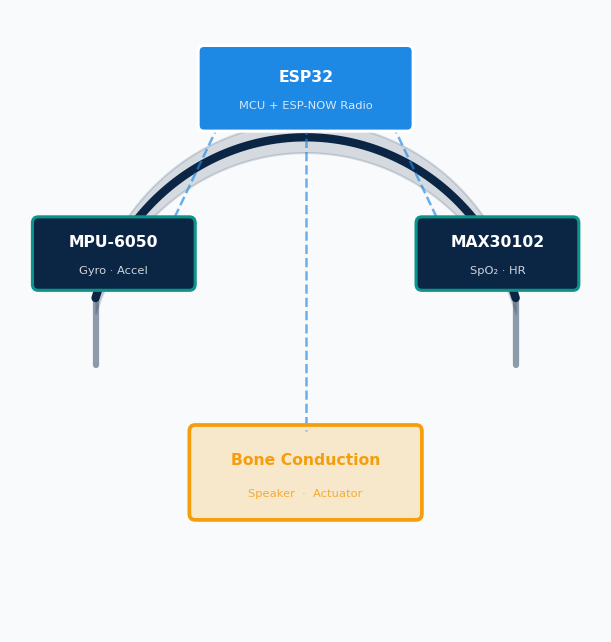
\includegraphics[width=\linewidth]{images/headband.png}
    \end{column}
    \begin{column}{0.54\textwidth}
      \textbf{\textcolor{sleepteal}{Sensors}}\\[0.5em]
      \begin{itemize}\setlength\itemsep{0.55em}
        \item \textbf{MPU-6050}\\
              {\small\textcolor{sleepgray}{3-axis gyroscope + accelerometer\\
              movement \& sleep stage detection}}
        \item \textbf{MAX30102}\\
              {\small\textcolor{sleepgray}{SpO\textsubscript{2} \& heart rate monitoring}}
      \end{itemize}
      \vspace{0.7em}
      \textbf{\textcolor{sleepteal}{Actuator}}\\[0.5em]
      \begin{itemize}\setlength\itemsep{0.4em}
        \item \textbf{Bone Conduction Speaker}\\
              {\small\textcolor{sleepgray}{Non-invasive therapeutic sound delivery}}
      \end{itemize}
      \vspace{0.7em}
      \textbf{\textcolor{sleepteal}{MCU:}} ESP32 (ESP-NOW radio)
    \end{column}
  \end{columns}
\end{frame}

% ── 6. GATEWAY DEVICE ─────────────────────────────────────────
\begin{frame}{Hardware — Gateway Device}
  \begin{columns}[c]
    \begin{column}{0.54\textwidth}
      \textbf{\textcolor{sleepteal}{Role:}} Bridge between headband and cloud\\[0.8em]
      \begin{itemize}\setlength\itemsep{0.65em}
        \item \textbf{ESP32} — dual role: ESP-NOW receiver + MQTT publisher
        \item \textbf{OLED Display} — real-time vitals readout at bedside
        \item \textbf{Wi-Fi} — relays sensor data to MQTT broker
        \item \textbf{Bluetooth} — one-time Wi-Fi setup via patient's smartphone
      \end{itemize}
      \vspace{0.7em}
      {\small\textcolor{sleepgray}{Deployable in hospital wards or home-care settings}}
    \end{column}
    \begin{column}{0.42\textwidth}
      \centering
      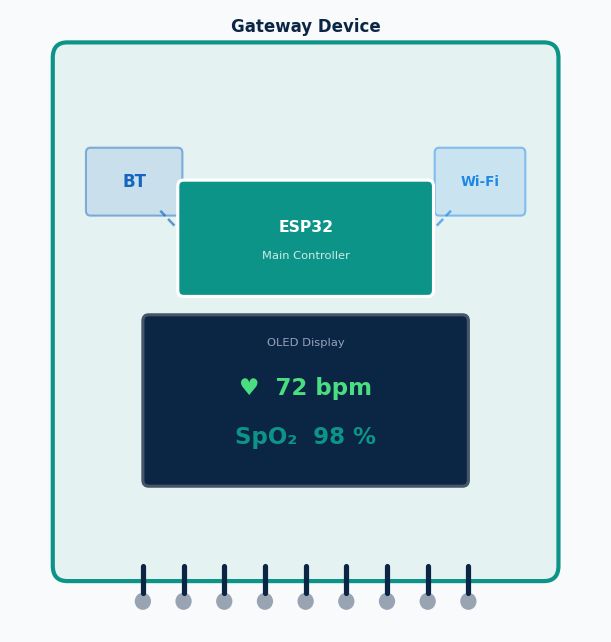
\includegraphics[width=\linewidth]{images/gateway.png}
    \end{column}
  \end{columns}
\end{frame}

% ── 7. COMMUNICATION PROTOCOLS ────────────────────────────────
\begin{frame}{Communication Protocols}
  \vspace{0.3em}
  \begin{columns}[T]
    \begin{column}{0.31\textwidth}
      \begin{alertblock}{\faBroadcastTower\enspace ESP-NOW}
        \textbf{Headband $\to$ Gateway}\\[0.5em]
        \begin{itemize}\setlength\itemsep{0.4em}
          \item Peer-to-peer, no router
          \item Ultra-low latency
          \item IEEE 802.11-based
        \end{itemize}
      \end{alertblock}
    \end{column}
    \begin{column}{0.31\textwidth}
      \begin{alertblock}{\faCloud\enspace MQTT}
        \textbf{Gateway $\to$ Cloud}\\[0.5em]
        \begin{itemize}\setlength\itemsep{0.4em}
          \item Lightweight pub/sub
          \item Minimal bandwidth
          \item QoS levels supported
        \end{itemize}
      \end{alertblock}
    \end{column}
    \begin{column}{0.31\textwidth}
      \begin{alertblock}{\faBluetoothB\enspace Bluetooth}
        \textbf{Phone $\to$ Gateway}\\[0.5em]
        \begin{itemize}\setlength\itemsep{0.4em}
          \item One-time Wi-Fi setup
          \item No extra hub needed
          \item Easy patient onboarding
        \end{itemize}
      \end{alertblock}
    \end{column}
  \end{columns}
\end{frame}

% ── 8. CLOUD & BACKEND ────────────────────────────────────────
\begin{frame}{Cloud \& Backend Stack}
  \centering
  \vspace{0.4em}
  \begin{tikzpicture}[
    layer/.style = {rectangle, rounded corners=5pt,
                    draw=cloudteal, fill=cloudteal!12,
                    text width=9.5cm, align=center, minimum height=0.85cm,
                    font=\small\bfseries, text=sleepnavy},
    arrv/.style  = {->, >=Stealth, line width=1.3pt, cloudteal}
  ]
    \node[layer] (mqtt) at (0,     0) {\faCloud\enspace    MQTT Broker — real-time sensor data ingestion};
    \node[layer] (db)   at (0, -1.35) {\faDatabase\enspace Time-Series Database — longitudinal patient storage};
    \node[layer] (api)  at (0, -2.70) {\faCode\enspace     Backend API — data access \& therapy command relay};
    \node[layer] (fe)   at (0, -4.05) {\faDesktop\enspace  Web Frontend — doctor's real-time dashboard};

    \draw[arrv] (mqtt) -- (db);
    \draw[arrv] (db)   -- (api);
    \draw[arrv] (api)  -- (fe);
  \end{tikzpicture}
\end{frame}

% ── 9. DOCTOR'S DASHBOARD ─────────────────────────────────────
\begin{frame}{Doctor's Dashboard}
  \begin{columns}[c]
    \begin{column}{0.48\textwidth}
      \centering
      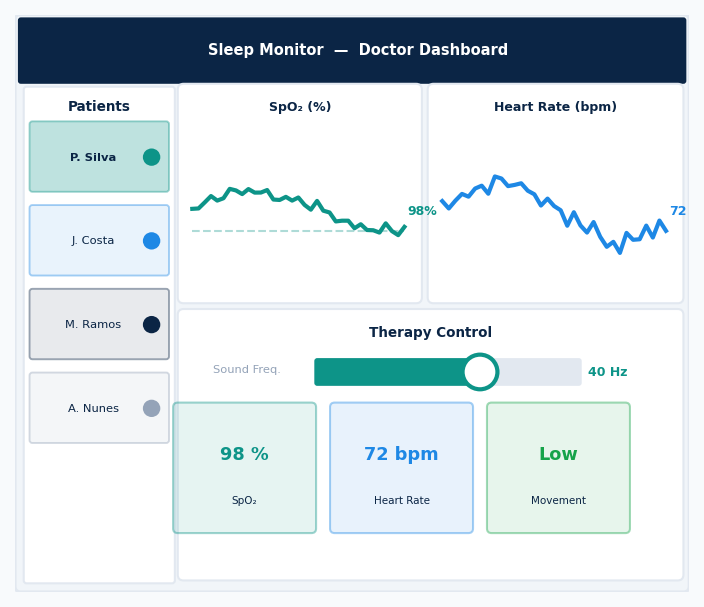
\includegraphics[width=\linewidth]{images/dashboard.png}
    \end{column}
    \begin{column}{0.48\textwidth}
      \begin{itemize}\setlength\itemsep{0.9em}
        \item[\textcolor{sleepteal}{\large\faChartLine}]
          \textbf{Real-time vitals} — SpO\textsubscript{2}, heart rate, movement
        \item[\textcolor{sleepteal}{\large\faHistory}]
          \textbf{Historical trends} — time-series view per patient
        \item[\textcolor{sleepteal}{\large\faSlidersH}]
          \textbf{Remote therapy control} — adjust bone conduction frequency
        \item[\textcolor{sleepteal}{\large\faUsers}]
          \textbf{Multi-patient} management from one interface
      \end{itemize}
    \end{column}
  \end{columns}
\end{frame}

% ── 10. DEMO PROTOTYPE ────────────────────────────────────────
\begin{frame}{Planned Prototype}
  \begin{columns}[T]
    \begin{column}{0.48\textwidth}
      \textbf{\textcolor{sleepteal}{\faCheckCircle\enspace Planned Features}}\\[0.6em]
      \begin{itemize}\setlength\itemsep{0.5em}
        \item Full sensor integration (MPU-6050, MAX30102)
        \item Bone conduction actuator
        \item ESP-NOW, MQTT \& Bluetooth links
        \item Cloud stack + doctor dashboard
        \item Remote frequency adjustment
      \end{itemize}
    \end{column}
    \begin{column}{0.48\textwidth}
      \textbf{\textcolor{warnambr}{\faTools\enspace Known Constraints}}\\[0.6em]
      \begin{itemize}\setlength\itemsep{0.5em}
        \item No integrated battery for demo
        \item No custom 3D-printed housing yet
        \item No clinical-scale load testing
        \item No sleep-stage ML classification
      \end{itemize}
    \end{column}
  \end{columns}
  \vspace{0.7em}
  \centering
  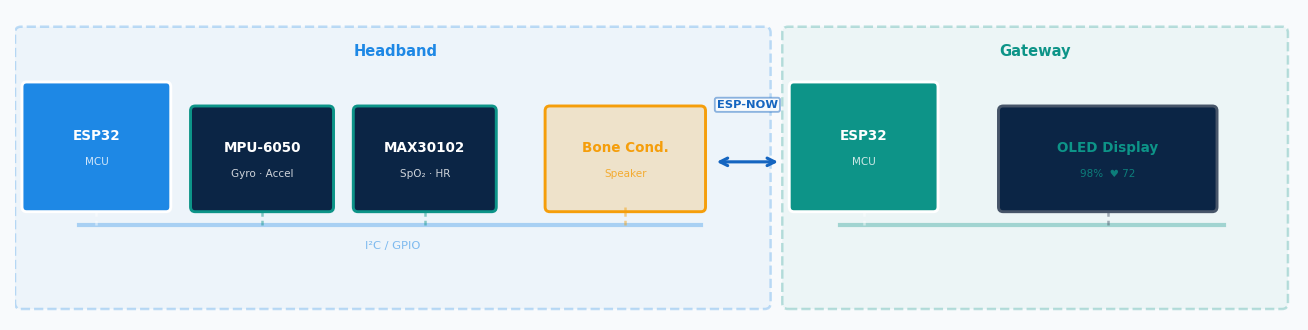
\includegraphics[width=\linewidth]{images/component_layout.png}
\end{frame}

% ── 11. CONCLUSIONS ───────────────────────────────────────────
\begin{frame}{Goals \& Expected Impact}
  \vspace{0.4em}
  \begin{columns}[T]
    \begin{column}{0.52\textwidth}
      \begin{itemize}\setlength\itemsep{1.0em}
        \item \textbf{Non-invasive} monitoring \& therapy will reduce patient discomfort
        \item \textbf{Remote control} will eliminate nighttime physical interventions
        \item \textbf{Scalable cloud} architecture designed for multi-ward deployment
        \item \textbf{Bluetooth setup} will lower barrier for home-care adoption
      \end{itemize}
    \end{column}
    \begin{column}{0.44\textwidth}
      \centering\vspace{0.4em}
      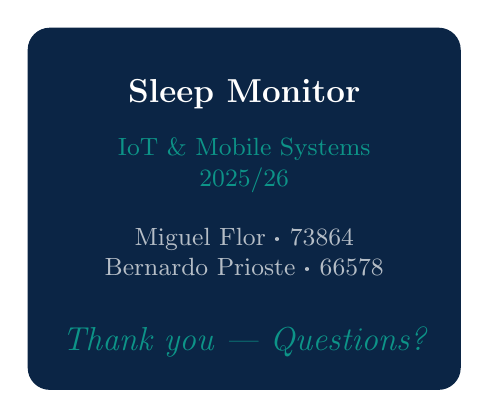
\begin{tikzpicture}
        \fill[sleepnavy, rounded corners=8pt] (0,0) rectangle (5.5,-4.6);
        \node[white,              font=\large\bfseries, align=center] at (2.75,-0.85)
          {Sleep Monitor};
        \node[sleepteal,          font=\small,          align=center] at (2.75,-1.75)
          {IoT \& Mobile Systems\\2025/26};
        \node[white!70!sleepnavy, font=\small,          align=center] at (2.75,-2.85)
          {Miguel Flor \textbf{·} 73864\\Bernardo Prioste \textbf{·} 66578};
        \node[sleepteal,          font=\large\itshape,  align=center] at (2.75,-4.0)
          {Thank you --- Questions?};
      \end{tikzpicture}
    \end{column}
  \end{columns}
\end{frame}

\end{document}
